\documentclass[a4paper,11pt]{article}
\usepackage[utf8]{inputenc}
\usepackage{minted}
\usepackage{subfig}
\usepackage{graphicx}
\begin{document}
\title{
    \textbf{Task 13 - Mandelbrot}
}
\author{Casper Kristiansson}
\date{\today}
\maketitle

\section*{Introduction}
Task thirteen of the course Programming II consisted of calculating the Mandelbrot set and visualizing it as an image. The Mandelbrot set is the complex numbers where the mathematical function $ f(z) = z^2 + c $ does not diverge to infinity when recursively iterate thought and remains in the bounded of the absolute value of two ($ |z| < 2 $).

\section*{Result}
The basics to create and visualize the Mandelbrot set consists of four different modules, one for the simple computations of complex numbers, one for calculating if a complex number is in the Mandelbrot set, one for creating each pixel in the image and lastly one for computation different colors. The author has also spent a lot of time mixing around with the program particularly the colors to create amazing looking patterns.

\subsection*{Complex numbers computations}
The first subtask of the problem is to create the different functions which should be able to perform a variety of different calculations on complex numbers. The author did have a bit of problem of creating the \textbf{sqr} method which should square a complex number.

\begin{figure}[H]
\begin{minted}{elixir}
  def new(r, i) do {r, i} end
  def add({r1, i1}, {r2, i2}) do {r1 + r2, i1 + i2} end
  def sqr({r, i}) do {r * r - i * i, 2 * r * i} end
  def abs({r, i}) do :math.sqrt(r * r + i * i) end
\end{minted}
\caption{Basic mathematical operations for complex numbers}
\label{Figure:1}
\end{figure}

\subsection*{Mandelbrot Calculations}
The next subtask of the problem is to implement the functions to check if a complex number converges using the $ f(z) = z^2 + c $ function when iterate through. It is also important that the number needs to remain inside the absolute value of two.

The function does this by creating a new complex number of zero and calling the function \textbf{test} recursively. It than adds the \textit{c} value to the square of the \textit{z} value. The function will continuously be called recursively until the max depth has been reached or if the absolute value is bigger than two.

If the value succeeds with reaching the maximum depth without its absolute value being bigger than two, results that the complex number is in the Mandelbrot set. The function will than return zero which will be represented by the center black areas (black is usually the default color but this could easily be changed).

\begin{figure}[H]
\begin{minted}{elixir}
  def mandelbrot(c, m) do
    z0 = Cmplx.new(0, 0)
    test(0, z0, c, m)
  end
  def test(i, _, _, m) when i >= m, do: 0
  def test(i, z, c, m) do
    if Cmplx.abs(z) < 2 do
      z = Cmplx.add(Cmplx.sqr(z), c)
      test(i + 1, z, c, m)
    else
      i
    end
  end
\end{minted}
\caption{Calculating if a complex number is in the Mandelbrot set}
\label{Figure:2}
\end{figure}

\subsection*{Main computation unit}
The next part of the problem consists of the main computation unit which will calculate if a certain value is in the Mandelbrot set and calculate a certain color for that specific position. The function receives the desired image width and height and a couple of other parameters. The method is split up into both \textbf{rows} and \textbf{row} where the rows make the correct pixel height call while the row function will calculate the width and find the correct color value of that specific position.

\begin{figure}[H]
\begin{minted}{elixir}
  def mandelbrot(width, height, x, y, k, depth) do
    trans = fn(w, h) ->
      Cmplx.new(x + k * (w - 1), y - k * (h - 1))
    end
    rows(width, height, trans, depth, [])
  end

  def rows(_, 0, _, _, rows), do rows end
  def rows(width, height, trans, depth, rows) do
    row = row(width, height, trans, depth, [])
    rows(width, height - 1, trans, depth, [row | rows])
  end

  def row(0, _, _, _, row), do row end
  def row(width, height, trans, depth, row) do
    complex = trans.(width, height)
    calculation = Brot.mandelbrot(complex, depth)
    color = Color.convert(calculation, depth)
    row(width - 1, height, trans, depth, [color | row])
  end
\end{minted}
\caption{Main computation unit}
\label{Figure:3}
\end{figure}

\subsection*{Coloring the Mandelbrot}
The last part of the problem is to visualize the Mandelbrot by representing it with RGB colors. Depending on what the main Mandelbrot function returns the color function will calculate a RGB value for that specific value. The author chooses to represent the numbers that is in the Mandelbrot set with black (RGB: 0, 0, 0). Figure four consists of two different Mandelbrot representation using the four main colors white, green, blue and red.

\begin{figure}[H]
\centering
\subfloat[\centering Green \& White]{{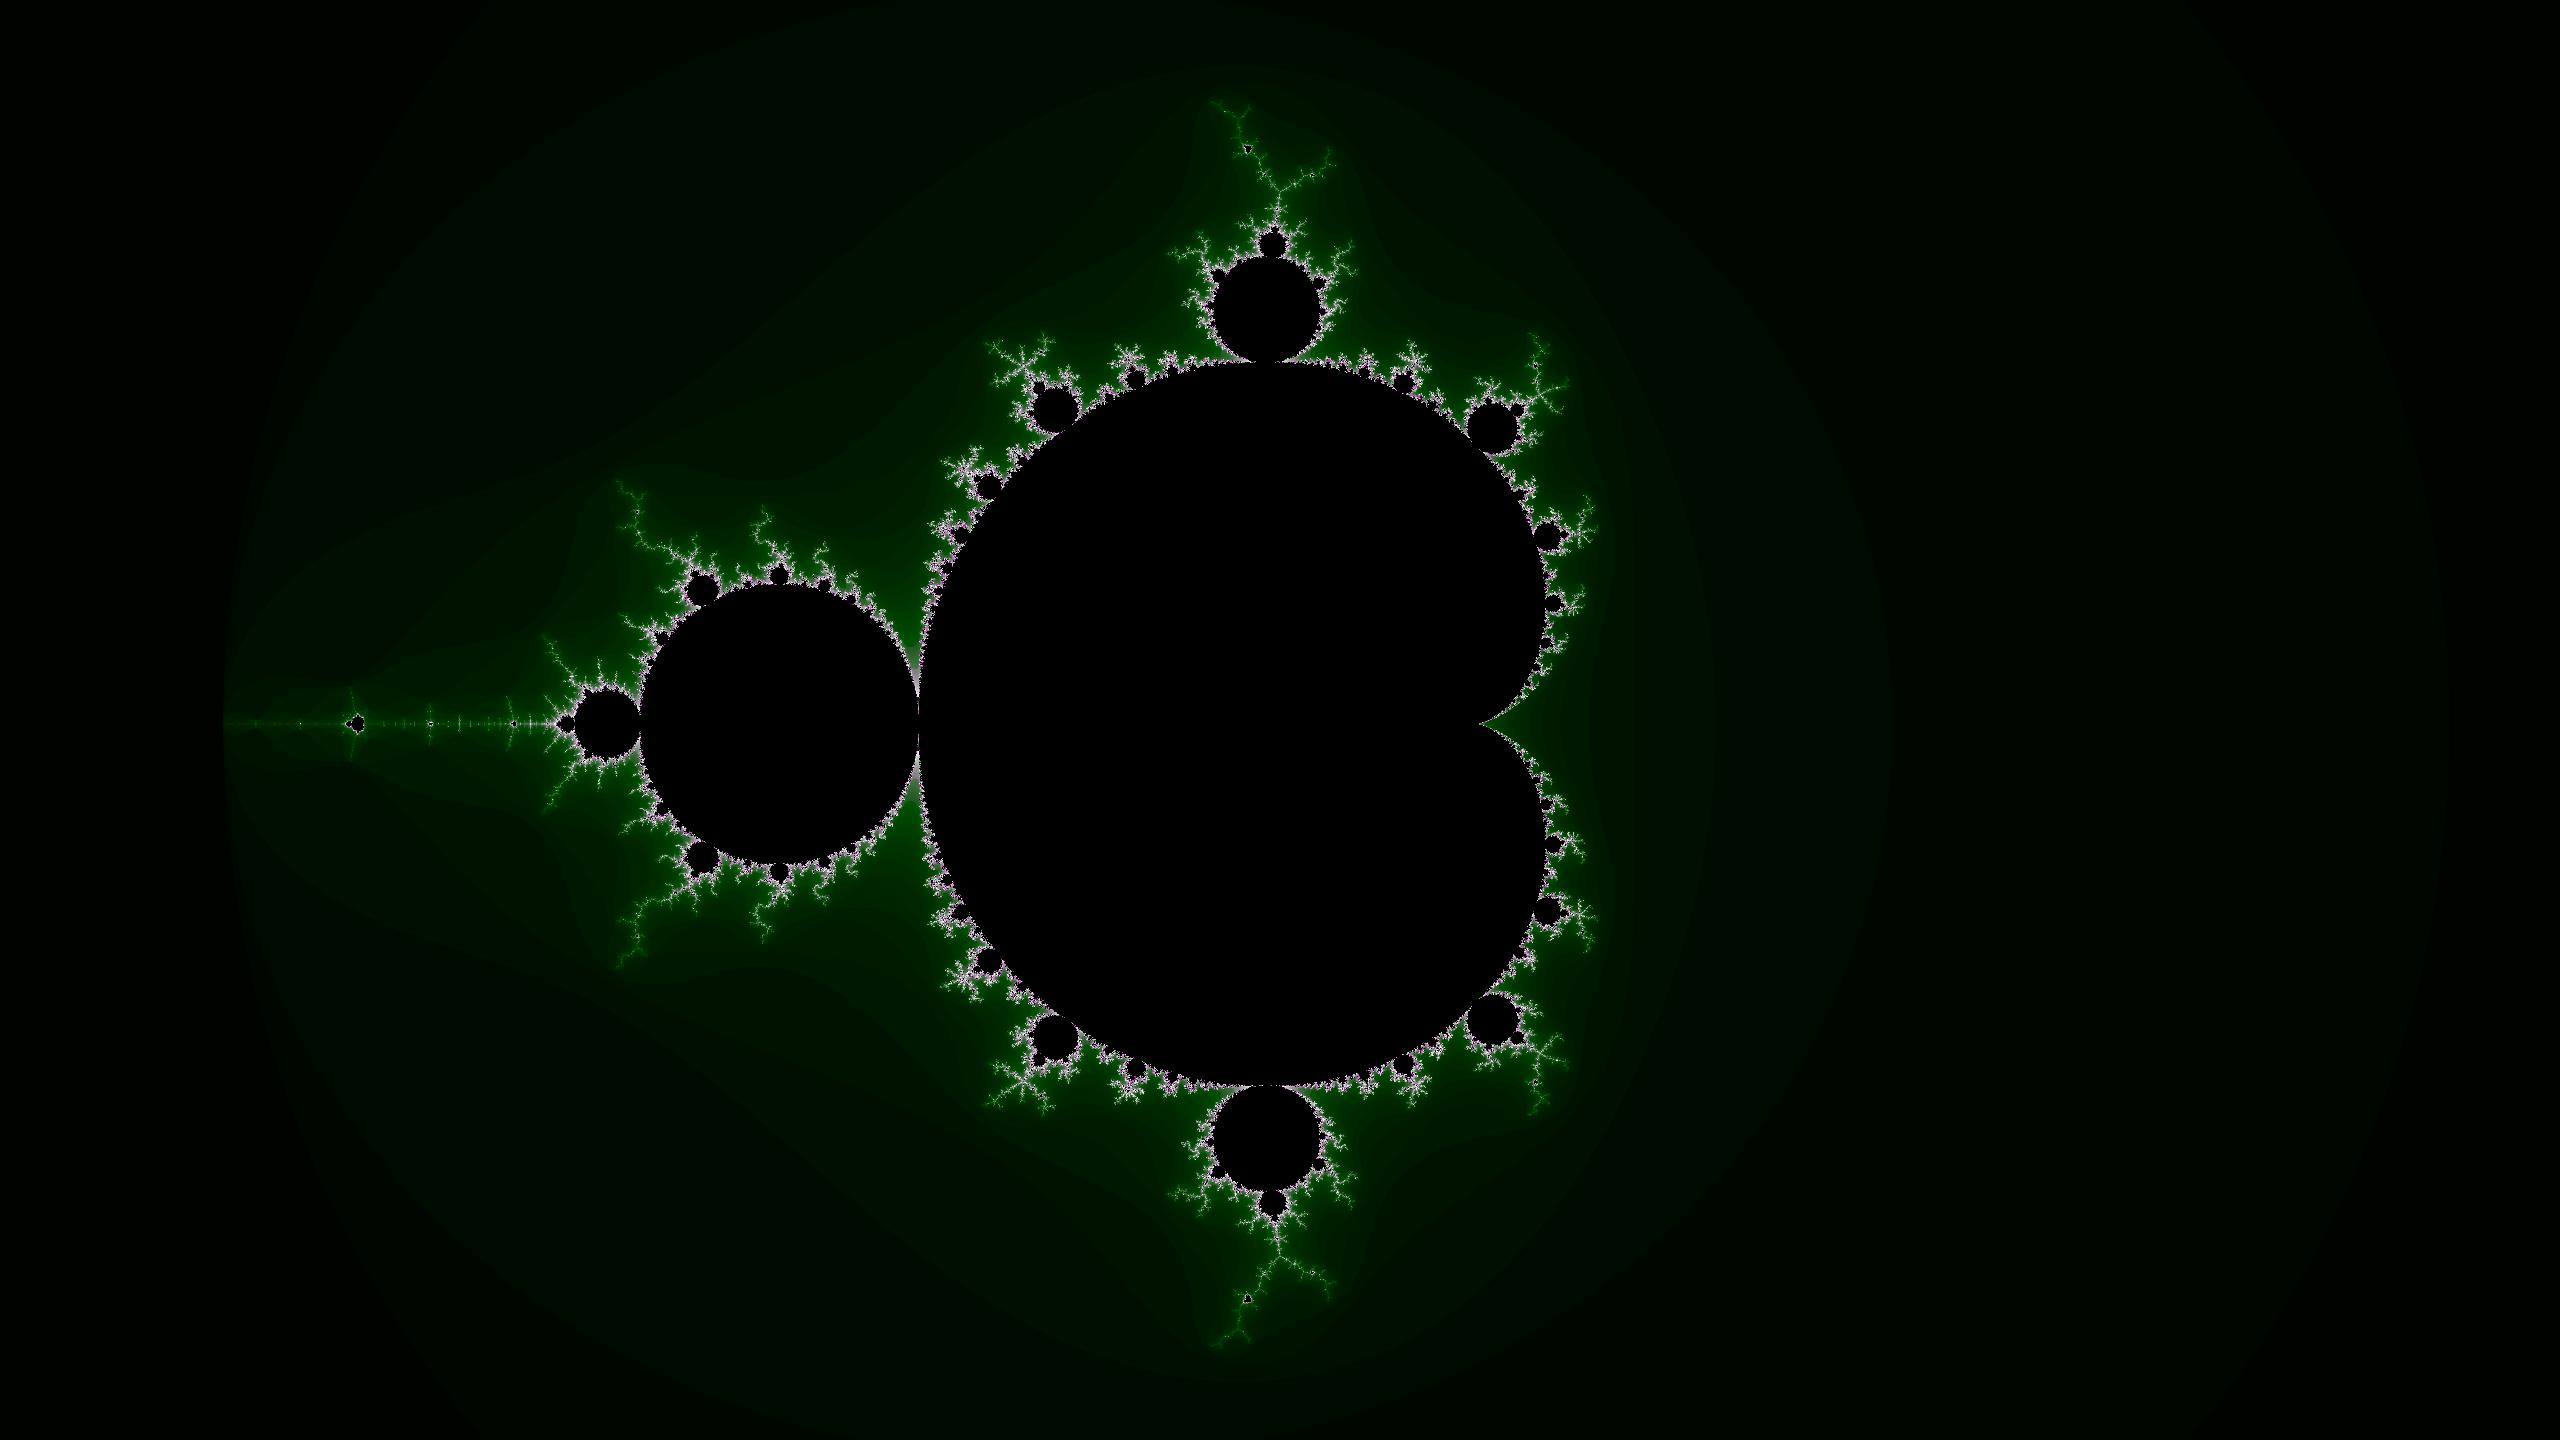
\includegraphics[width=5cm]{Task 13 Images/Green & White.jpg} }}%
\qquad
\subfloat[\centering Blue \& Purple]{{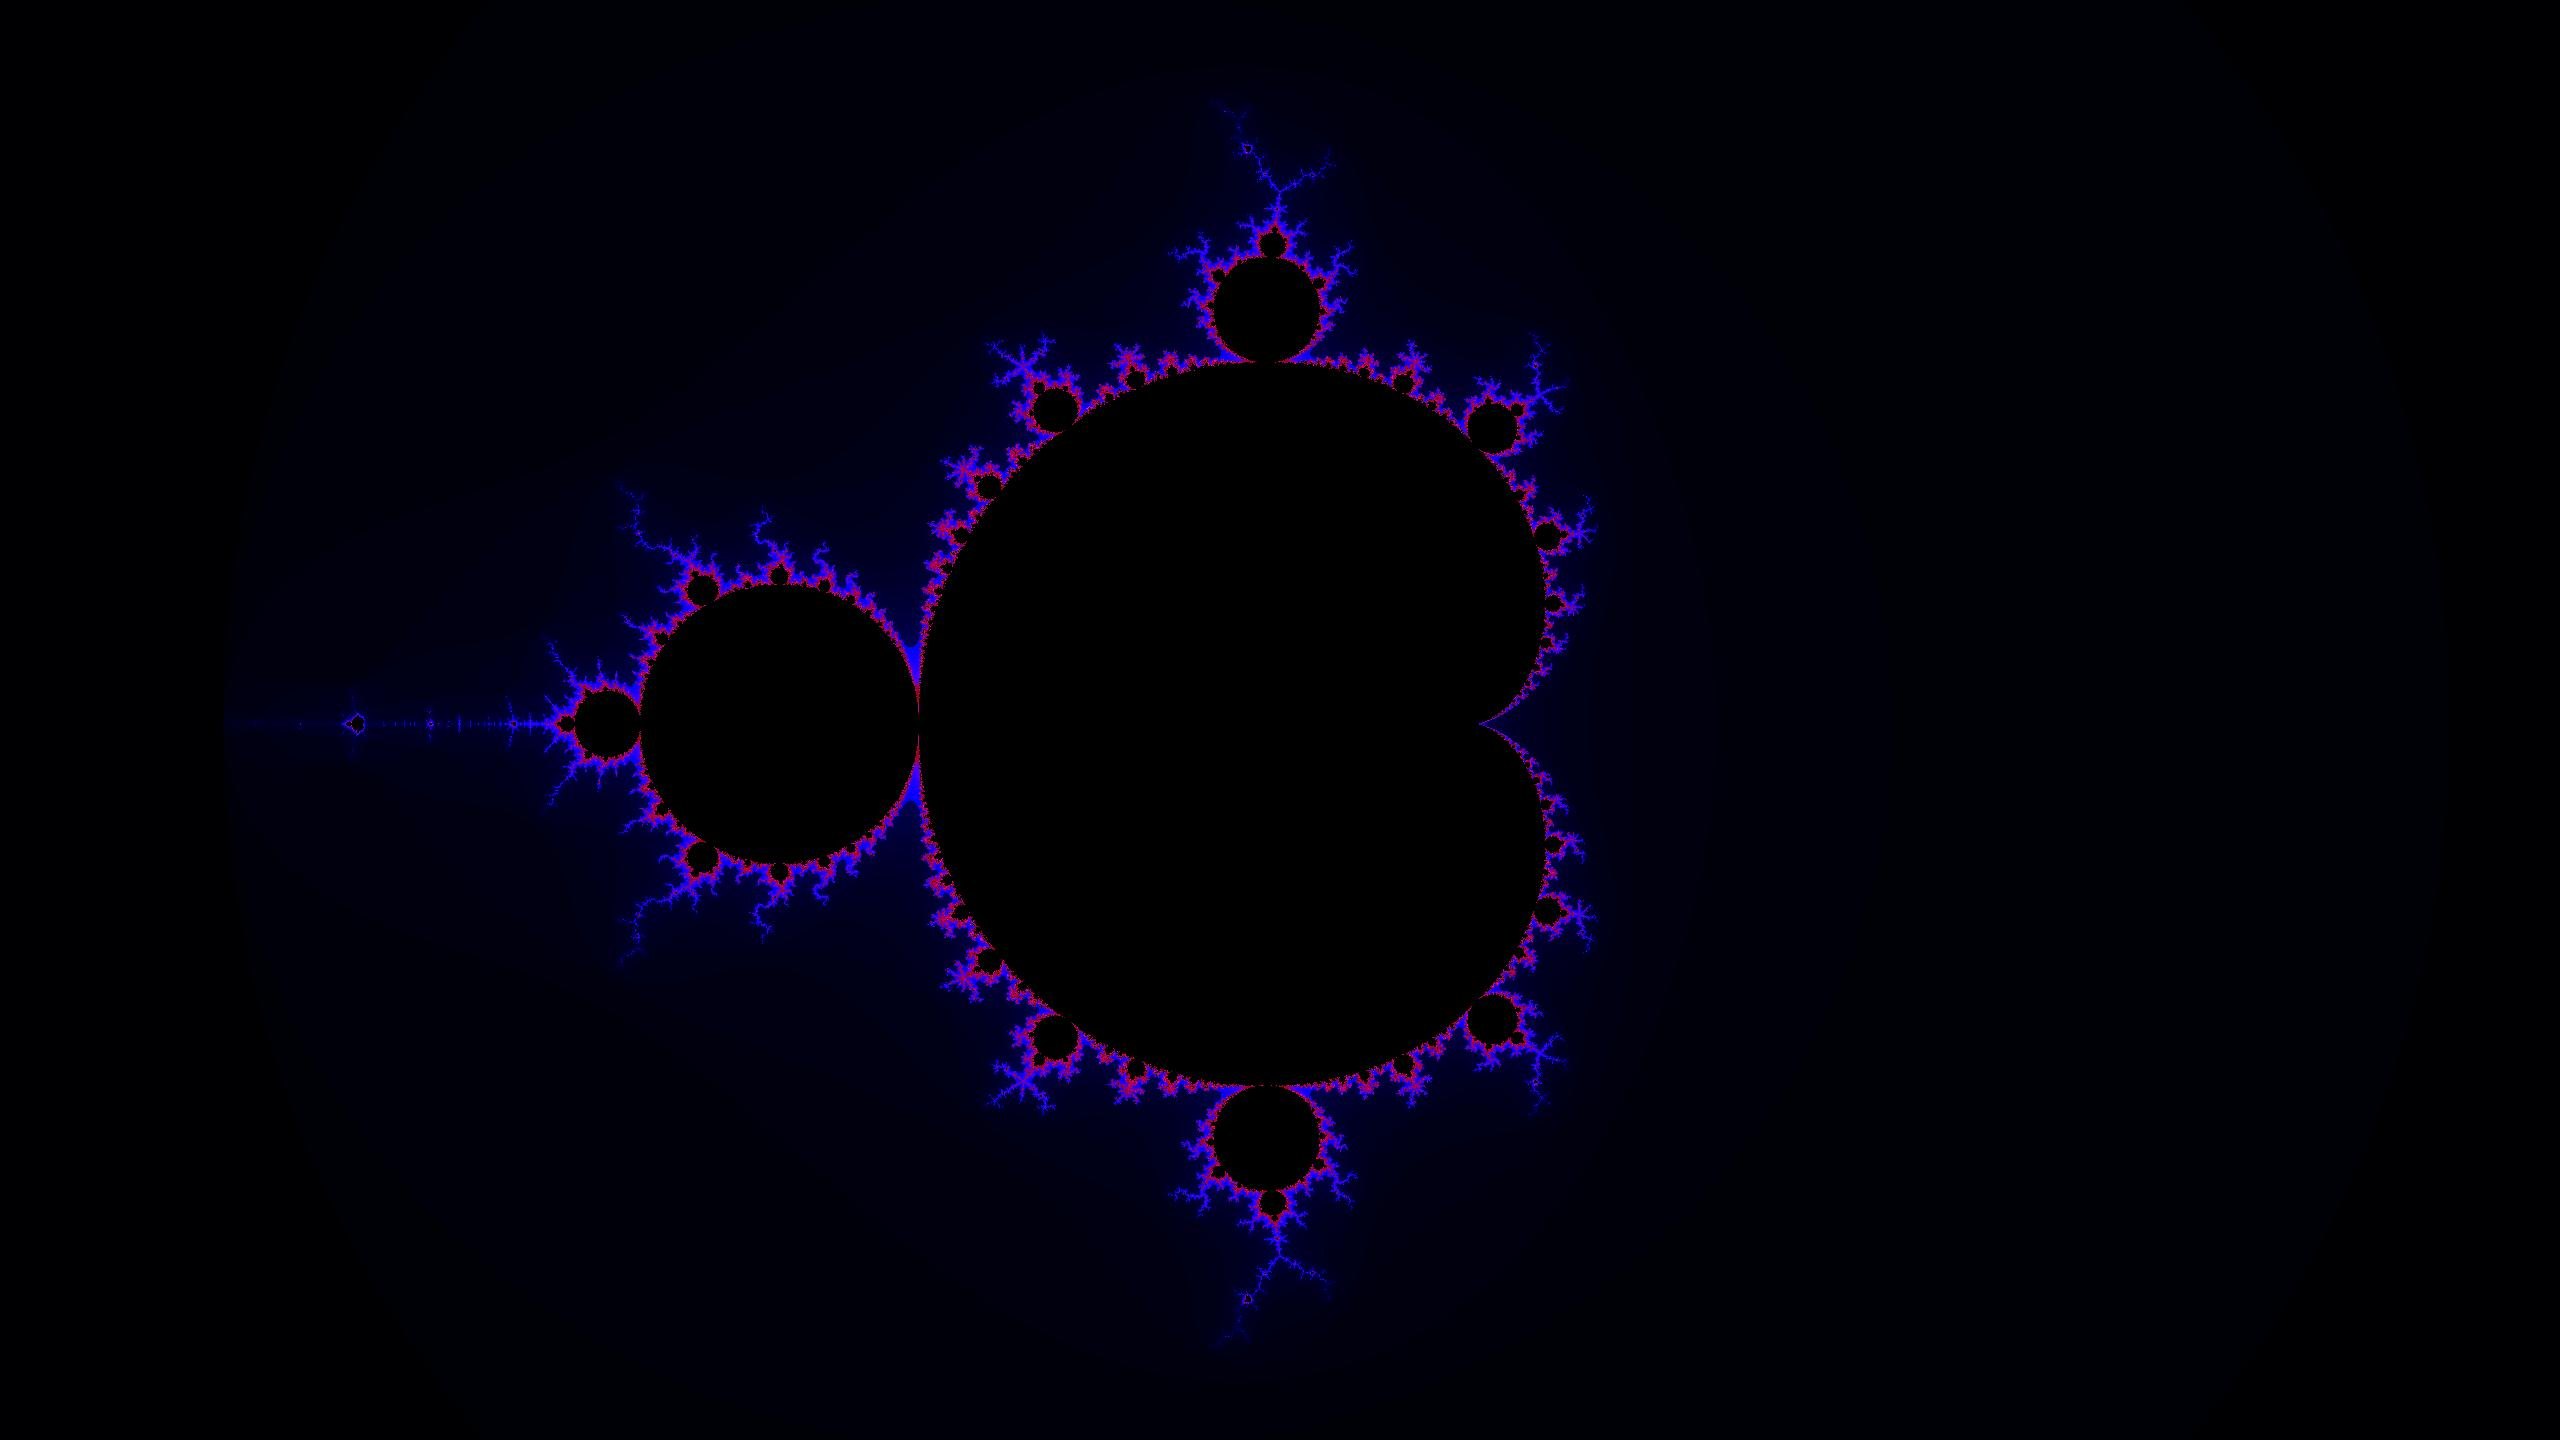
\includegraphics[width=5cm]{Task 13 Images/Blue & Purple.jpg} }}%
\caption{The result images of the visualization of the Mandelbrot set}
\label{Figure:4}
\end{figure}

The function \textbf{convert} calculates a RGB offset, \textbf{y}, which is responsible for returning specific values depending on what max value it receives. Then the method calls a specific color pattern with that offset. The author took a lot of time with experimenting and creating a lot of several types of color patterns. For example, figure five consist of the green and white pattern.

\begin{figure}[H]
\begin{minted}{elixir}
  def convert(depth, max) do
    a = (depth / max) * 4
    x = trunc(a)
    y = trunc(255 * (a - x))
    green_white(x, y)
  end
  
  def green_white(x, y) do
    case x do
      0 ->
        cond do
          y < 85 ->
            {0, y, 0}
          y < 120 ->
            {y - 50, y, y - 50}
          true ->
            {y, y, y}
        end
      1 ->
        {y, y, y}
      2 ->
        {255 - y, y, 255 - y}
      3 ->
        {255, y, 255}
      4 ->
        {255 - y, 255, 255 - y}
    end
  end
\end{minted}
\caption{Coloring method which returns a RGB value for a specific pixel}
\label{Figure:5}
\end{figure}

\section*{Discussion}
The author took a lot time to play around with the start values \textit{x0, y0, xn}. These values would both change the position and size of the Mandelbrot figure. The finale value that the author choose for these was $ x0 = -2.4, y0 = 1.3, xn = 2.2 $. Those values positioned the Mandelbrot in the center of the image with a good sizing where all the bright colors are shown. The author also chooses to represent all the Mandelbrot calculations with a depth of 256.

The author also created a python script which simply and automatically converted the images from ppm format to jpg. The last part of this report includes the python script and an image dump of all the Mandelbrot images that the author created.

\begin{figure}[H]
\begin{minted}{python}
  from PIL import Image
  import os
  import time
  while True:
    for file in os.listdir():
      if '.ppm' in file:
        im = Image.open(file)
        im.save(f'{os.path.splitext(file)[0]}.jpg')
        os.remove(file)
        print(f'Saved: {file}')
    time.sleep(5)
\end{minted}
\caption{Converting a ppm file to a jpg file}
\label{Figure:6}
\end{figure}

\begin{figure}[ht]
\centering
\subfloat[\centering Blue \& Purple]{{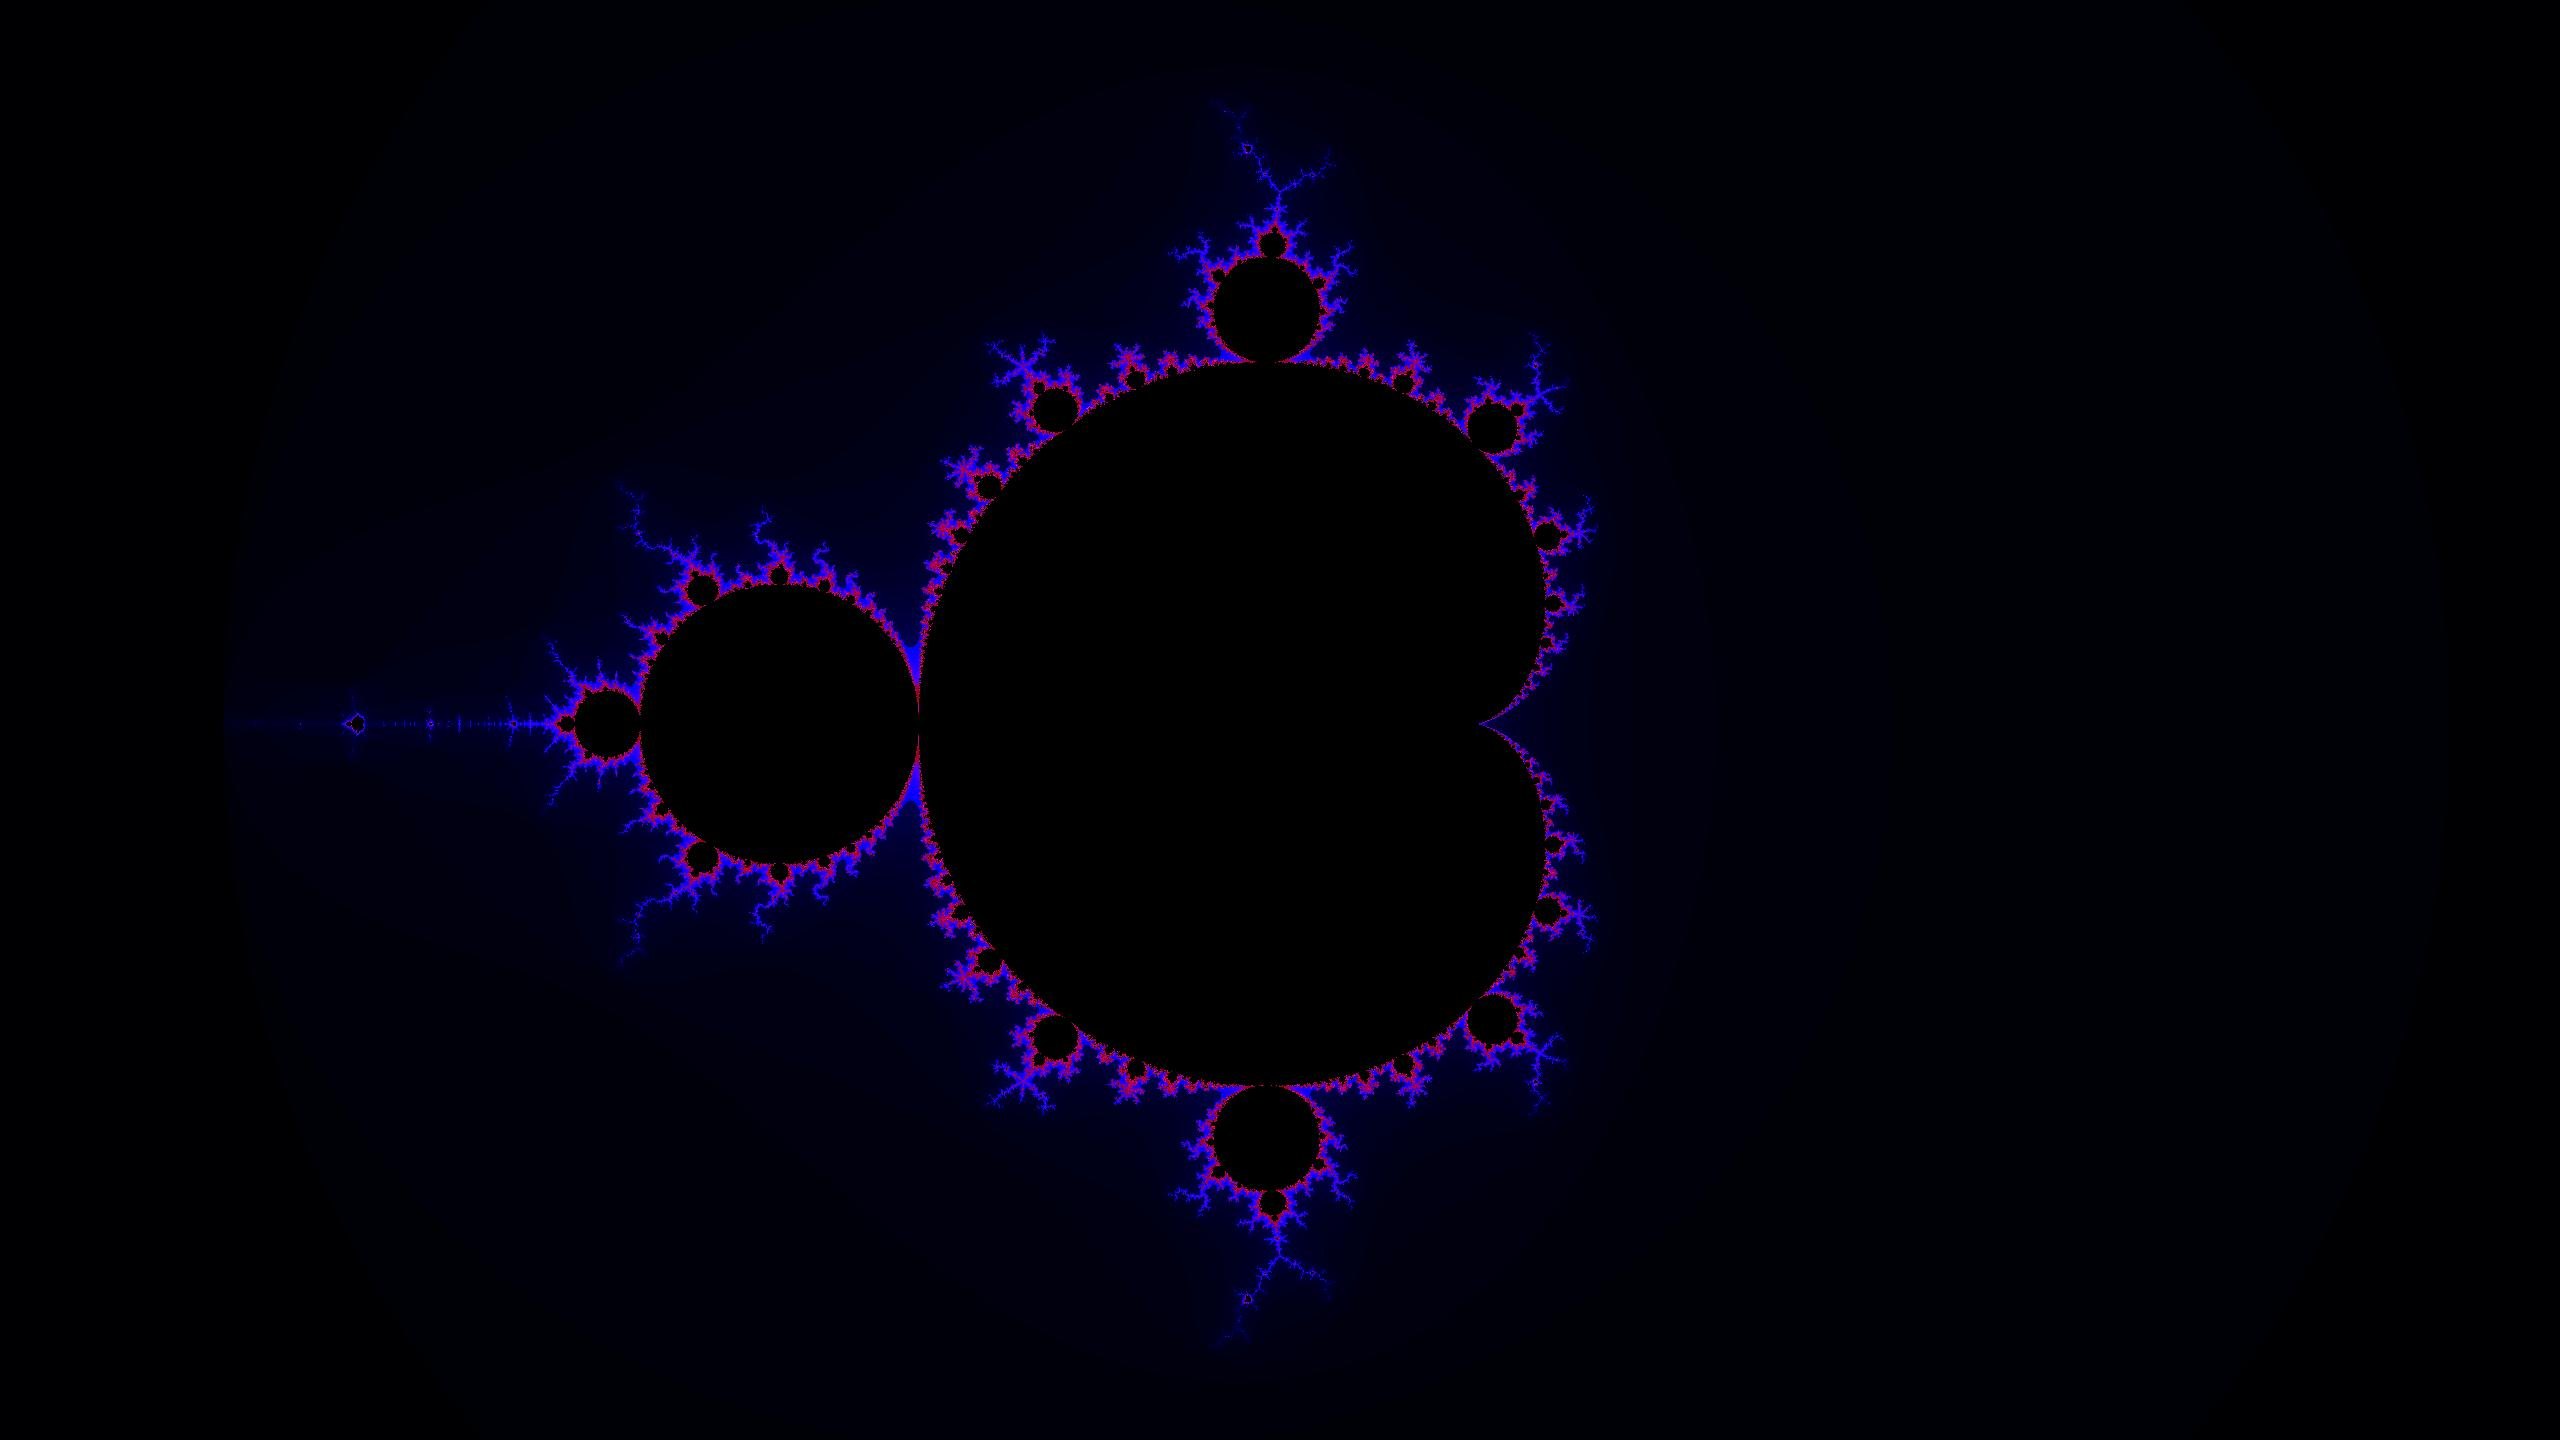
\includegraphics[width=5cm]{Task 13 Images/Blue & Purple.jpg} }}%
\qquad
\subfloat[\centering Red \& Yellow]{{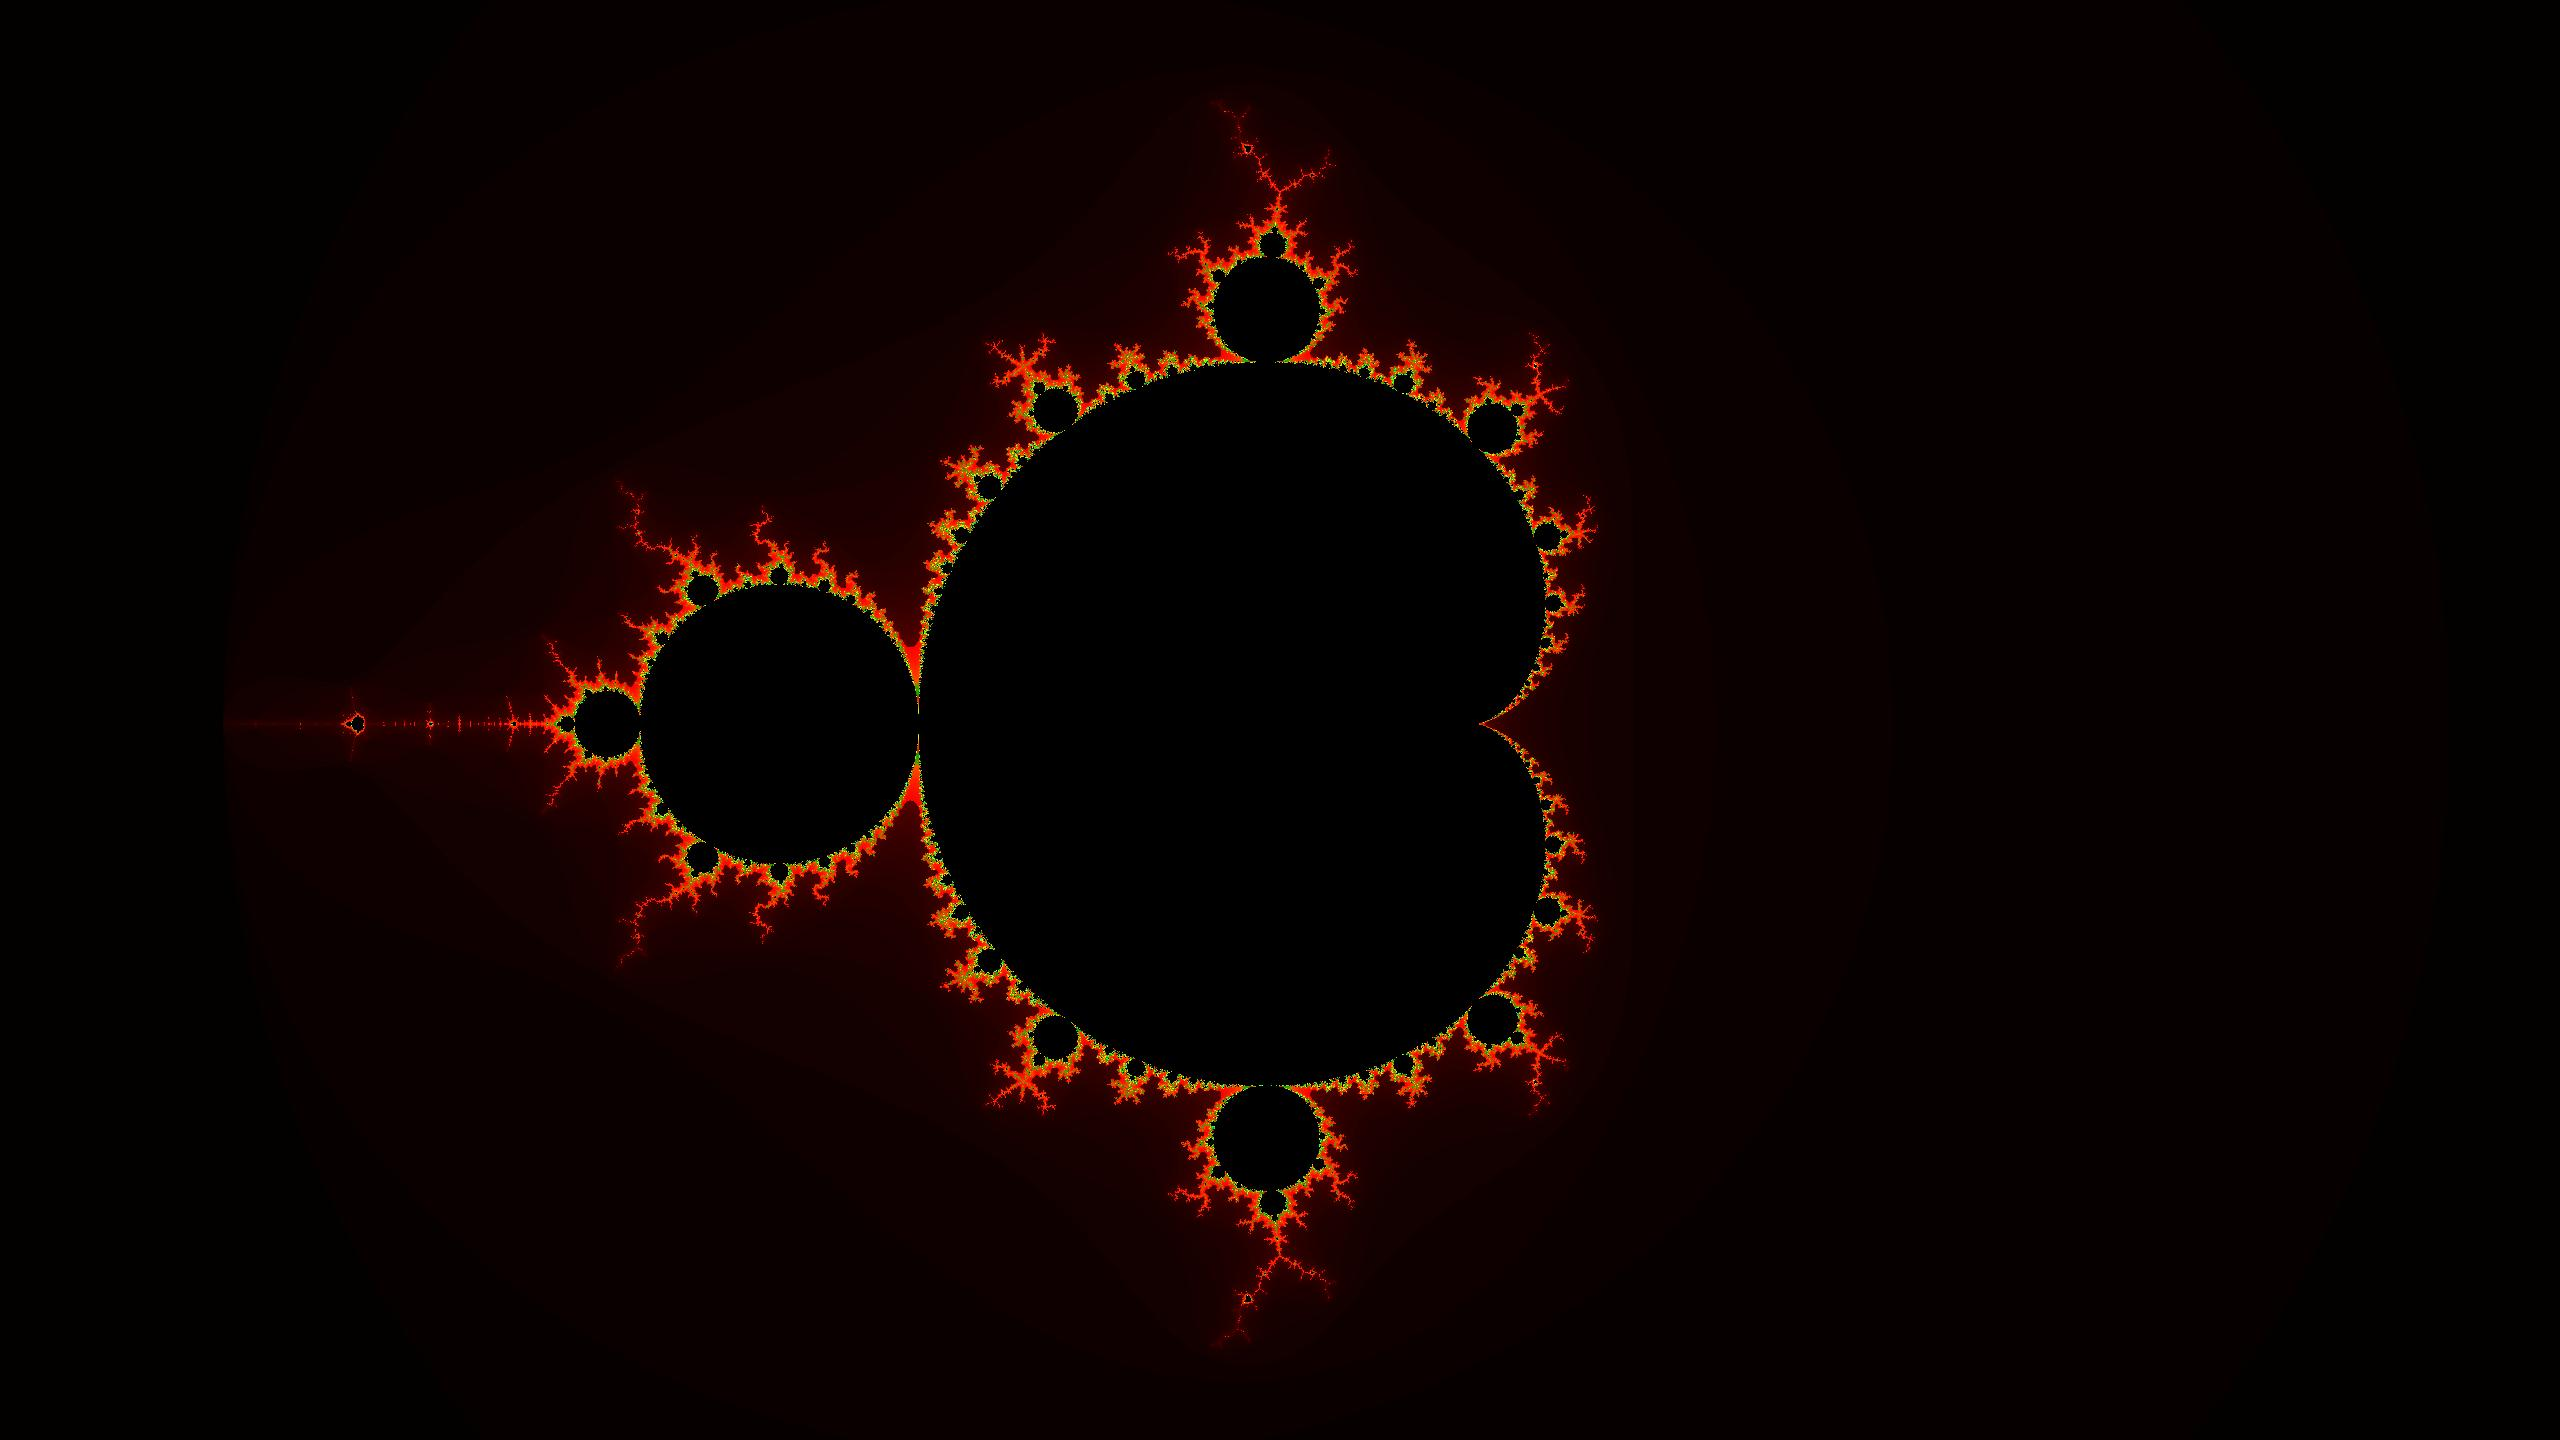
\includegraphics[width=5cm]{Task 13 Images/Red & Yellow.jpg} }}%
\qquad
\subfloat[\centering Red \& Pink]{{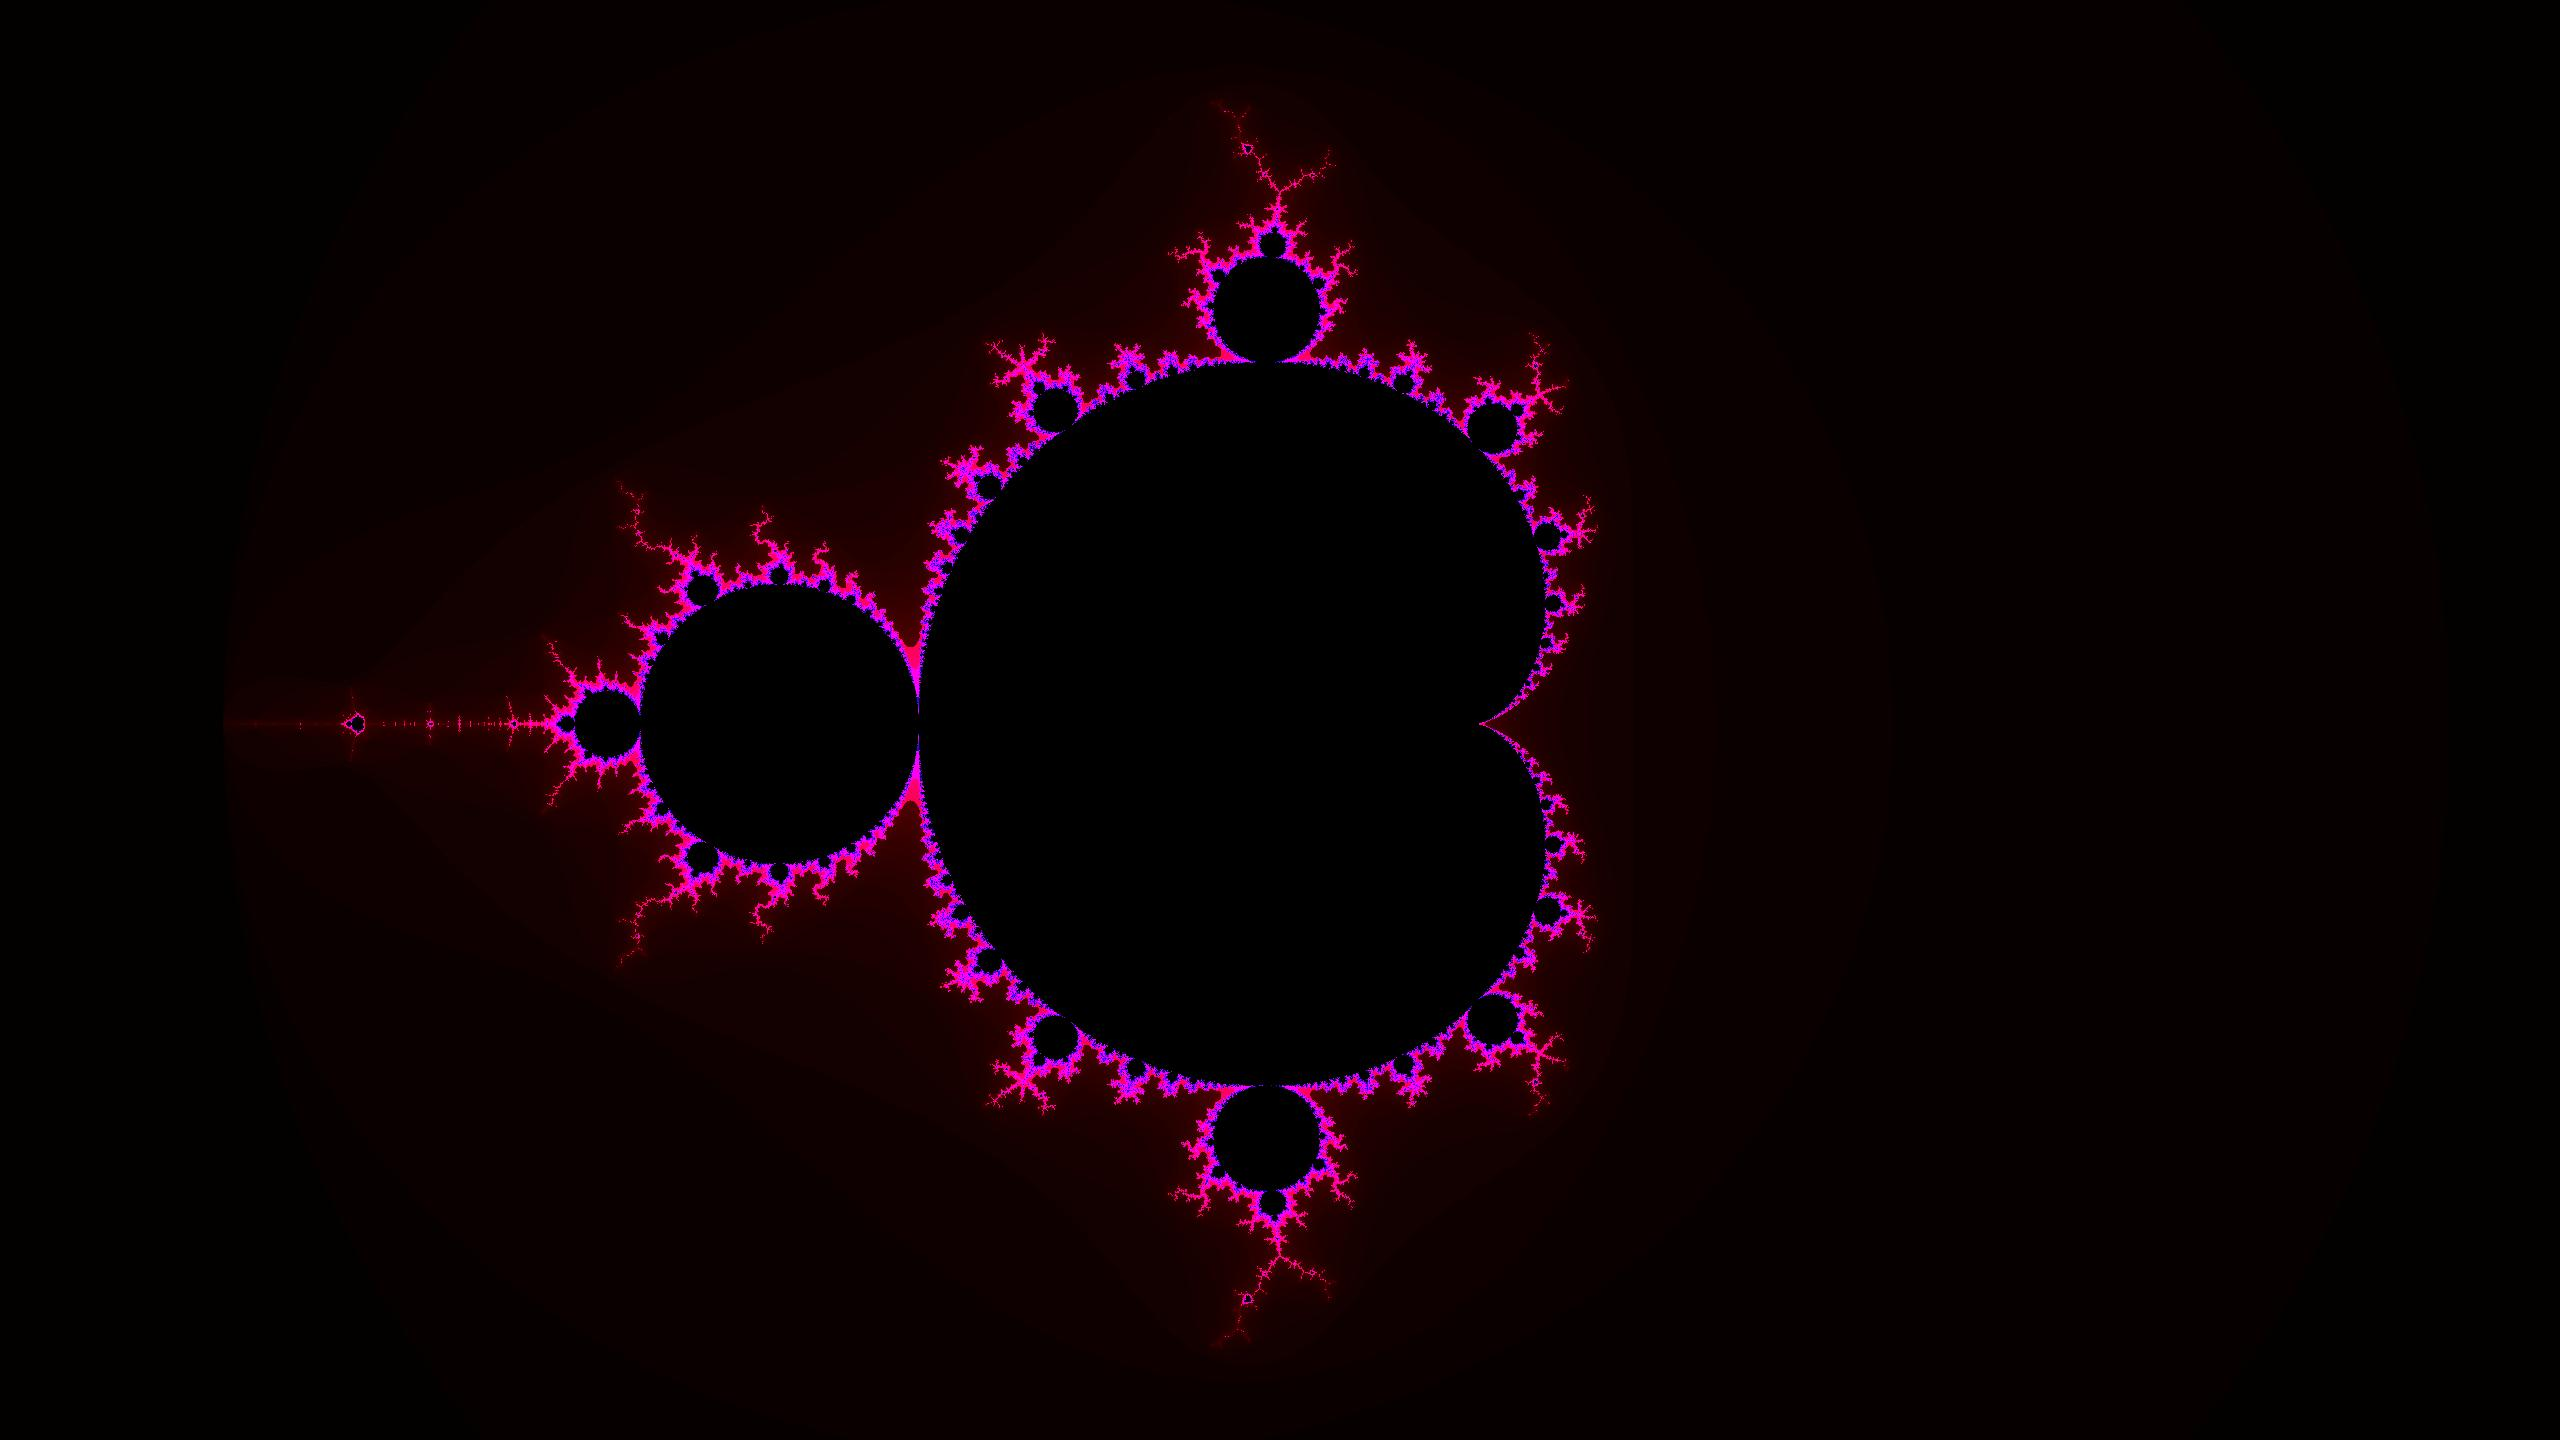
\includegraphics[width=5cm]{Task 13 Images/Red & Pink.jpg} }}%
\qquad
\subfloat[\centering Blue \& Green]{{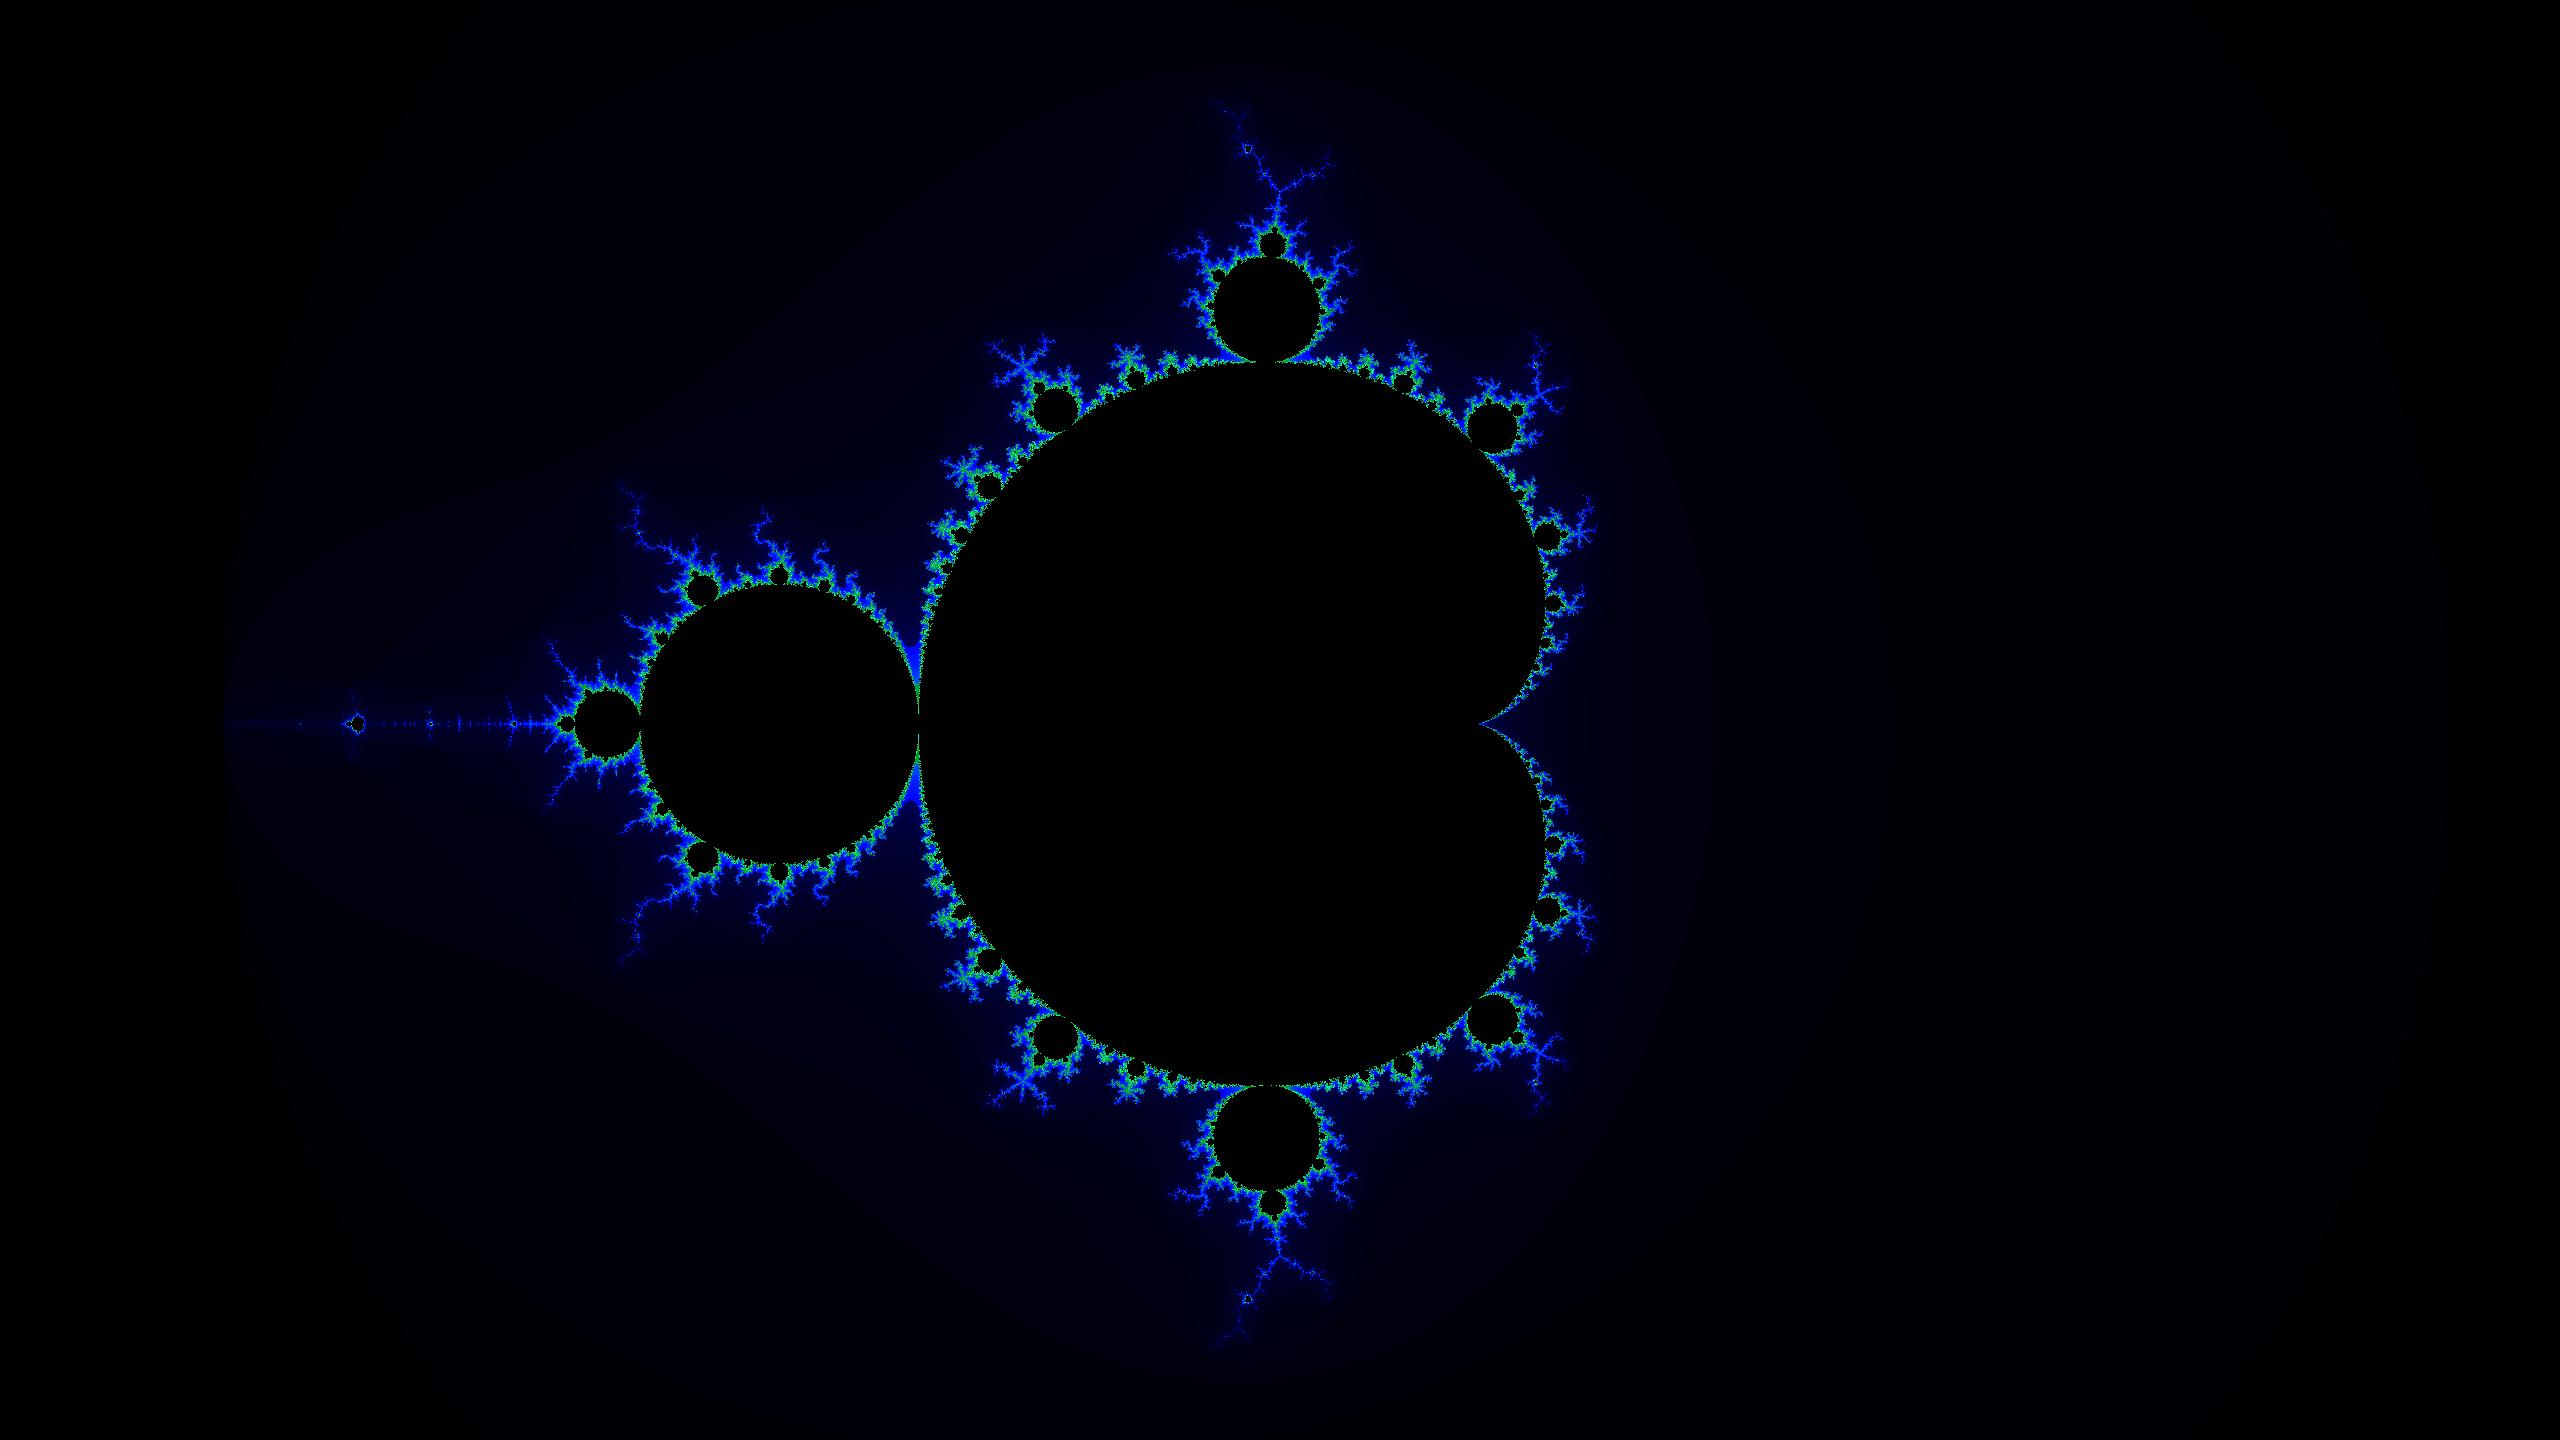
\includegraphics[width=5cm]{Task 13 Images/Blue & Green.jpg} }}%
\qquad
\subfloat[\centering Zoomed Branches]{{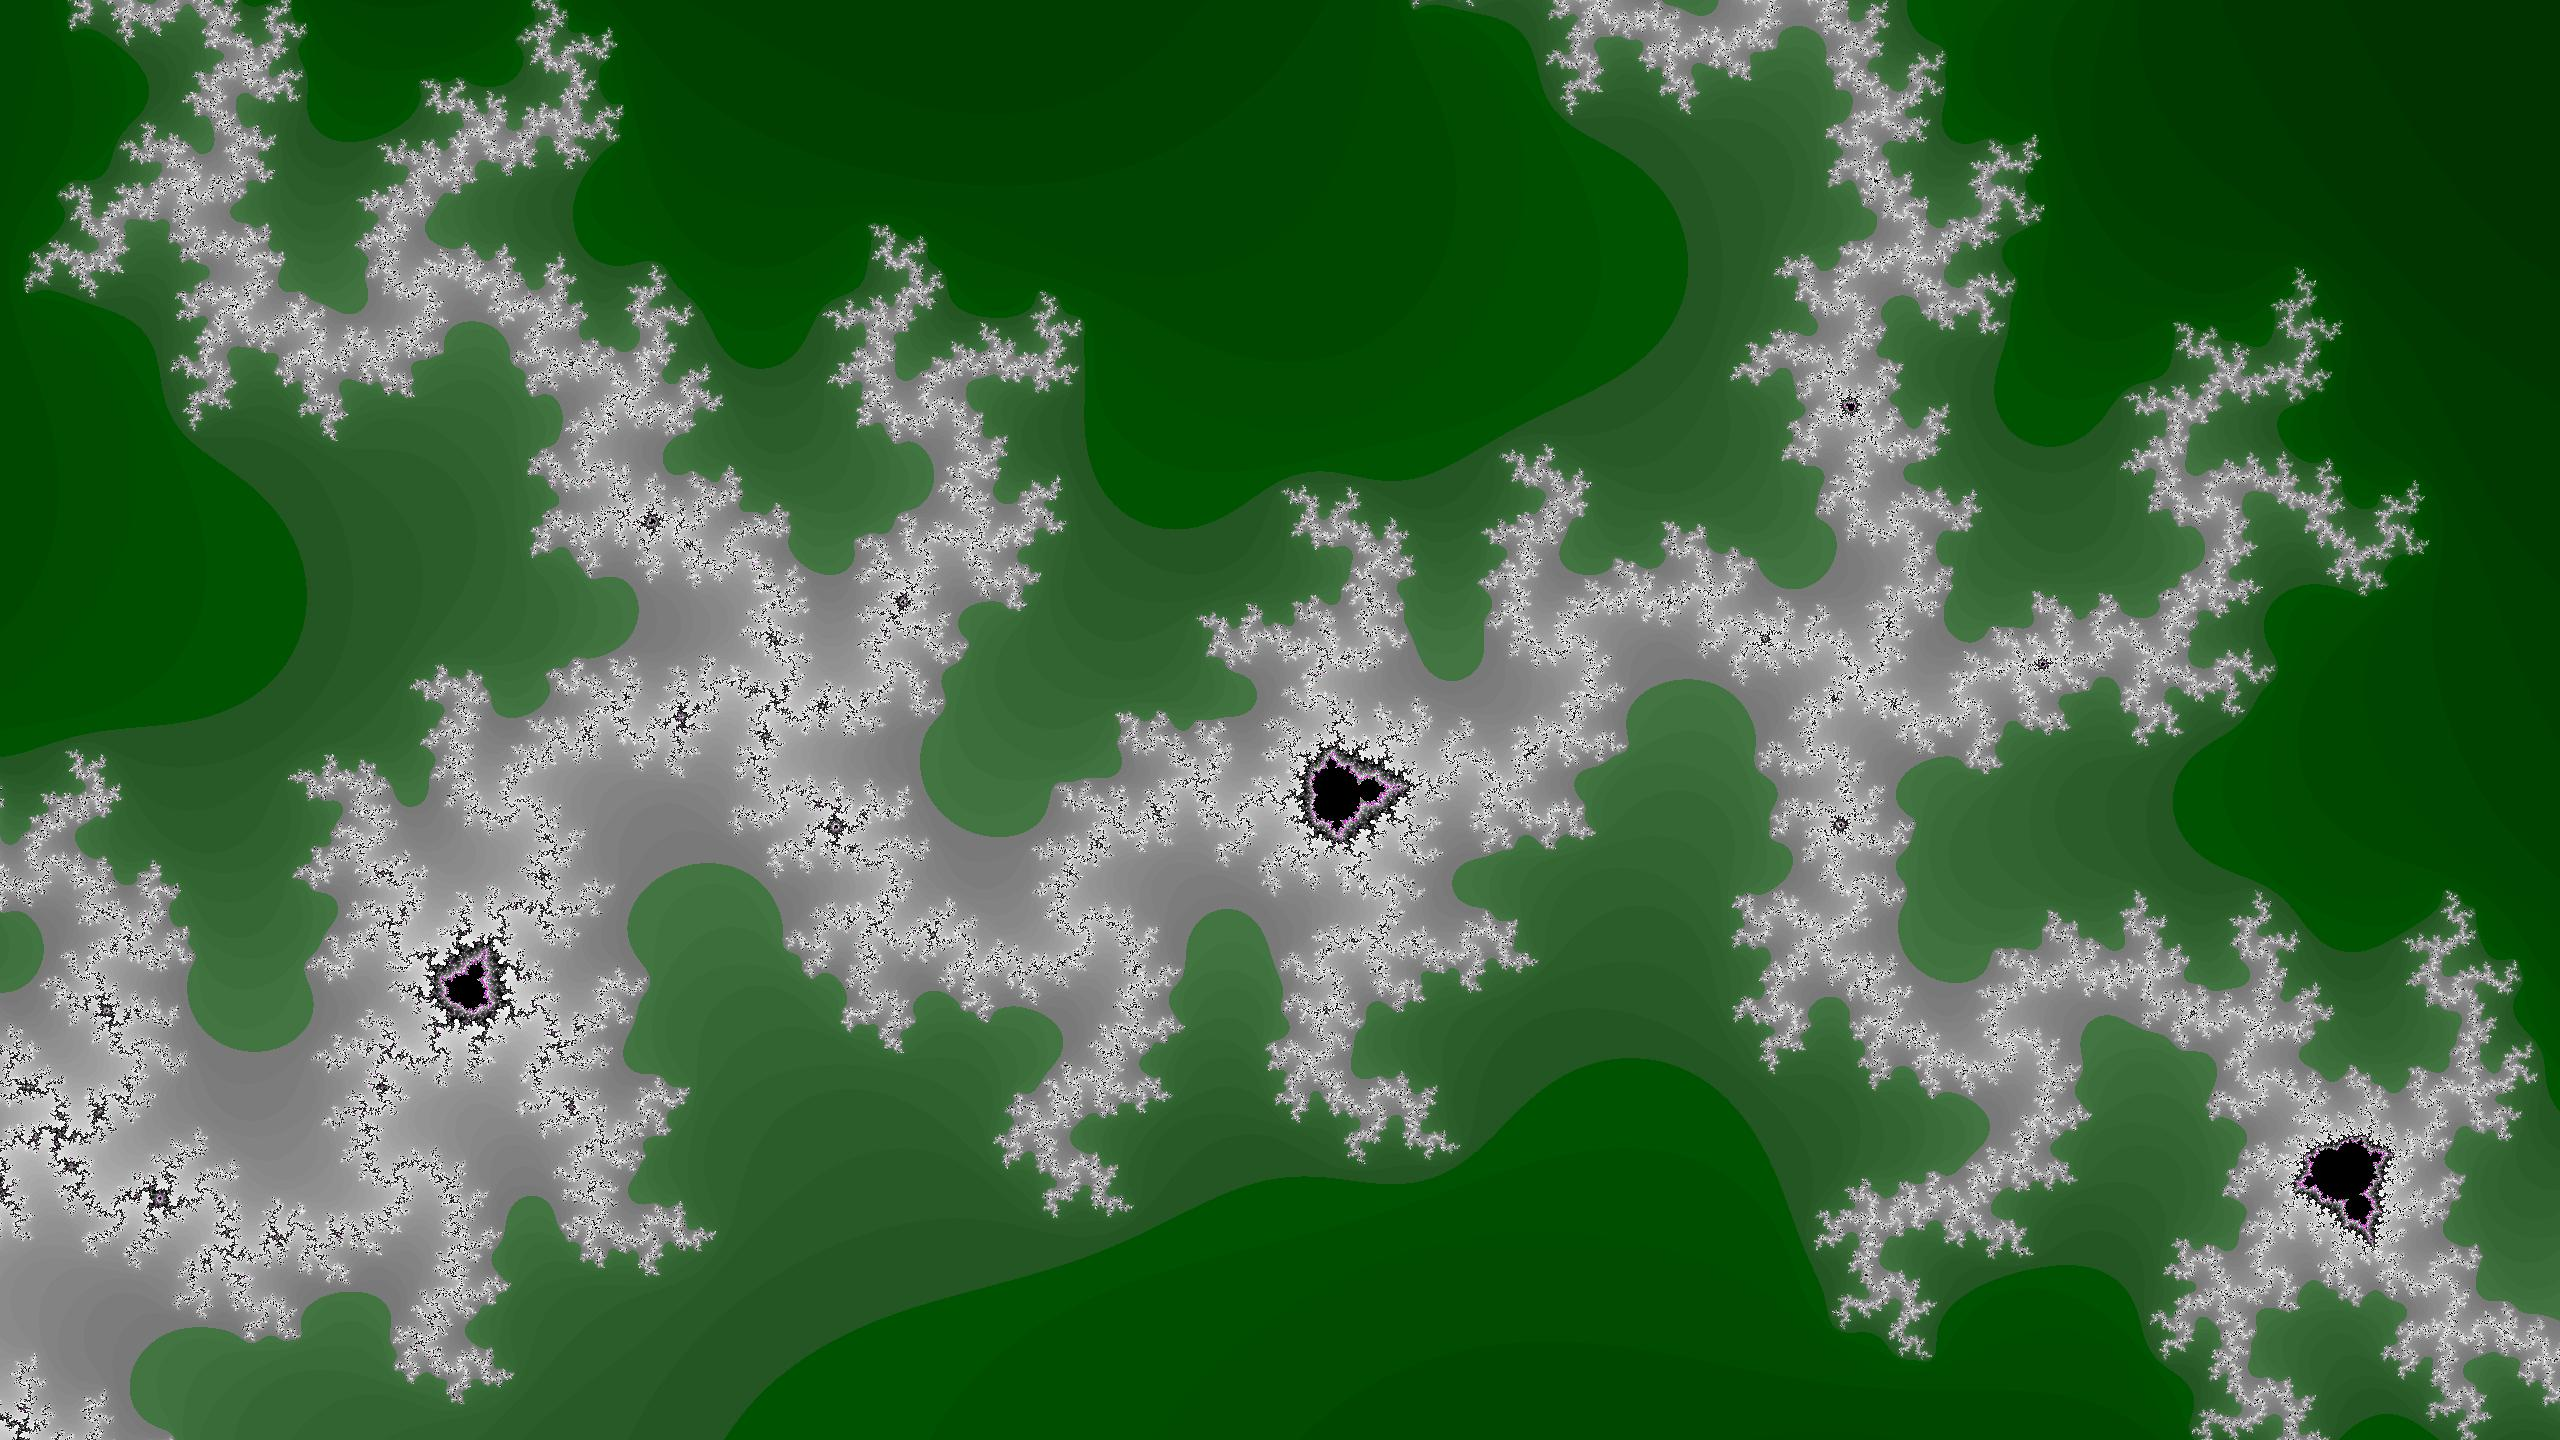
\includegraphics[width=5cm]{Task 13 Images/Zoomed Branches.jpg} }}%
\qquad
\subfloat[\centering Zoomed Circles]{{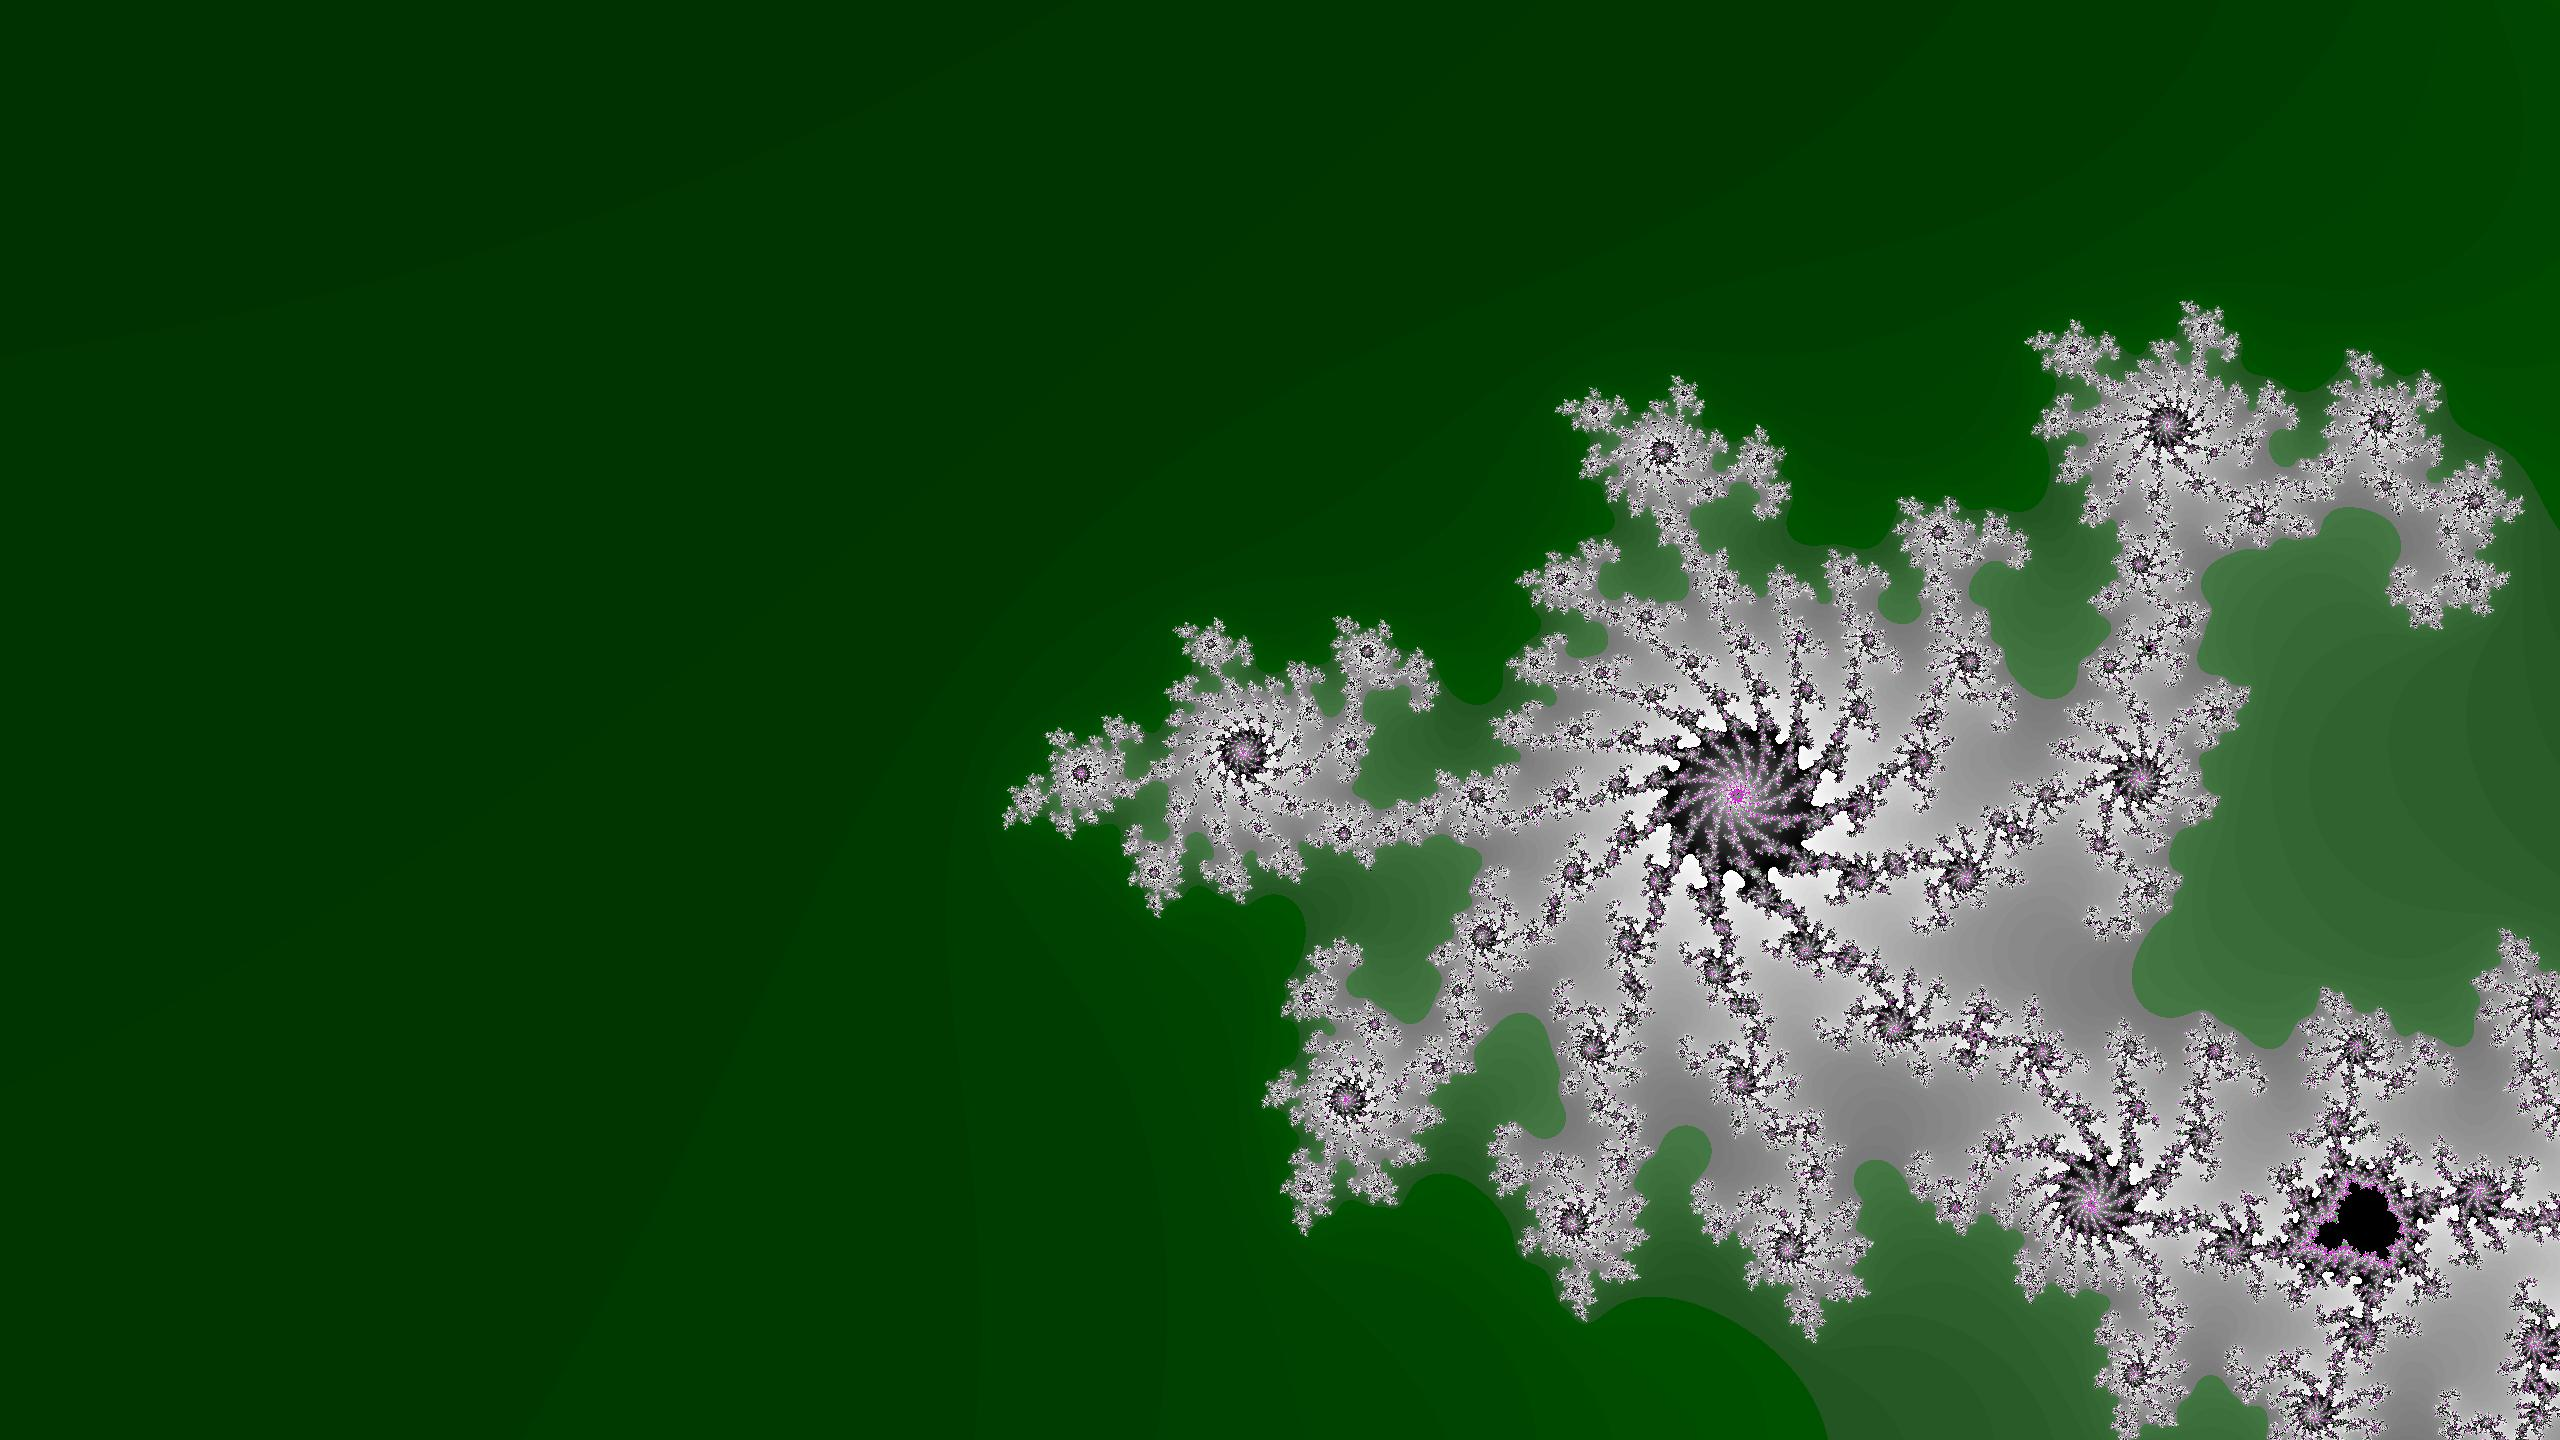
\includegraphics[width=5cm]{Task 13 Images/Zoomed Circles.jpg} }}%
\caption{Image dump}
\label{Figure:7}
\end{figure}

\end{document}